\chapter*{Ergebnisse des GeomInt-Vorhabens}

%\begin{wrapfigure}{l}{0.4\textwidth}
%\vspace{-5mm}
%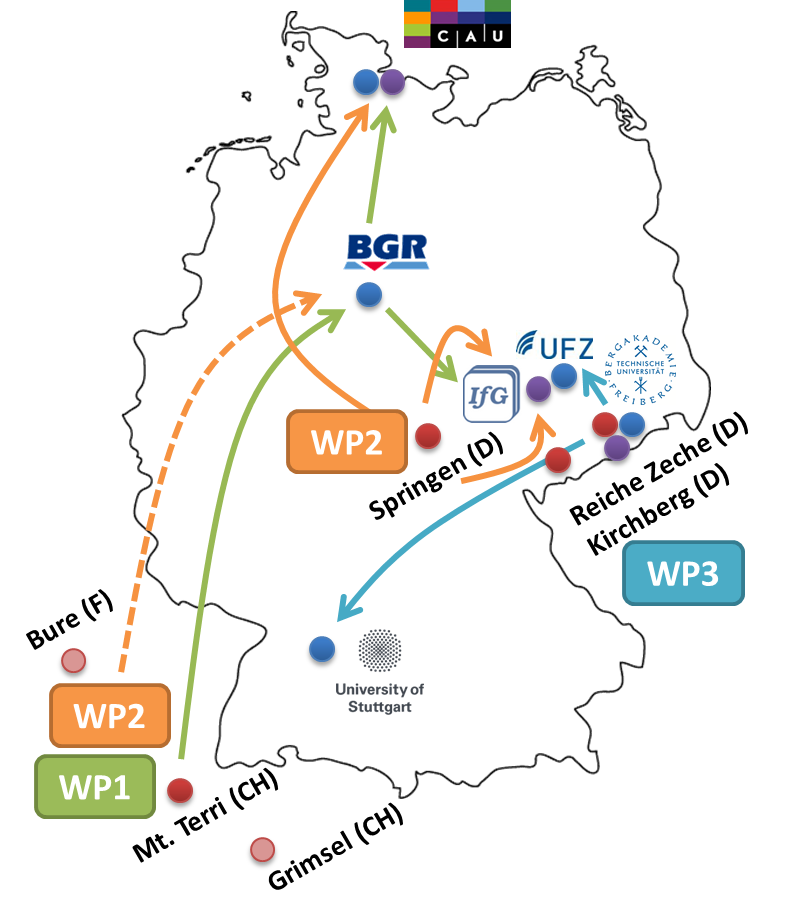
\includegraphics[width=0.39\textwidth]{figures/geomint-all.png}
%\caption{GeomInt Projekt-Geographie}
%\label{fig:geomint-geographie}
%\end{wrapfigure}
Die wichtigsten erreichten Ergebnisse des GeomInt-Vorhabens werden entsprechend der Arbeitspakete (APs) im Folgenden zusammengestellt (Abschn. \ref{sec:wp1}-\ref{sec:wp3}). Eine geografische Verortung der Aktivitäten ist in der Abb. \ref{fig:appraoch} dargestellt. Die APs sind eng verknüpft mit den Untertagelaboren (URLs) Mt. Terri (AP1/AP2), Springen (AP2) und Reiche Zeche (AP3). Aus den URLs stammt das Probenmaterial für die geotechnischen Labore in Freiberg (TUBAF), Kiel (CAU) und Leipzig (IfG) (Abschn. \ref{sec:exp}). Daten aus In-situ-Versuchen in Mt. Terri (BGR) und der Grube Springen (IfG) fanden Eingang in die Modellierungsplattform des GeomInt-Vorhabens (Abschn. \ref{sec:mod}) unter Koordination des UFZ an der sich alle Projektpartner beteiligt haben.
Als Synthese-Instrument wurden sogenannte Modell-EXperimente (MEX) definiert, in denen experimentelle und Modellierungsarbeiten von Beginn an systematisch zusammengeführt wurden (Abschn. \ref{sec:syn}). 

Bisher wurden bereits 12 GeomInt-Publikationen in internationalen Fachzeitschriften und 3 in Proccedings veröffentlicht, 3 Manuskripte sind zur Begutachtung eingereicht und 6 Manuskripte sind in Vorbereitung für die Geo:N Topical Collection in Environmental Earth  Sciences\footnote{\url{https://link.springer.com/journal/12665/topicalCollection/AC_efd2f04ddbcca9be8213d04bf1e1fd42}}. Eine umfassende Darstellung der Ergebnisse des Gesamtvorhabens befindet sich im vorliegenden GeomInt-Buch.
%======================================================================================
\section*{AP1: Wegsamkeiten durch Quell- und Schrumpfungsprozesse}
\label{sec:wp1}

Zur Gewinnung von Probenmaterial wurden im Felslabor Mt. Terri von der BGR zwei Bohrkampagnen durchgeführt. Neben der geologischen Charakterisierung der Kerne wurde das Gestein vom Bohrloch aus durch elektrische Resistivitätstomographie und Miniseismik untersucht. Wissenschaftler der BGR und der CAU Kiel führten die Probenahme durch, bei der mehr als 20 Meter Kernproben von Opalinuston gewonnen wurden. Diese Kerne sind in Laborversuchen weiter analysiert worden, um Diskontinuitäten zu untersuchen. 
%\begin{comment}
\begin{wrapfigure}{l}{0.33\textwidth}
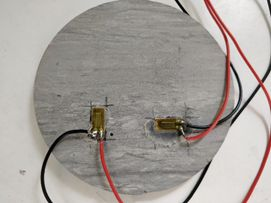
\includegraphics[width=0.3\textwidth]{figures/CAU_shrink_exp_01.jpg}
\caption{Messung von Quell-Dehnungen in und senkrecht zur Schichtungsebene (CAU)}
\label{fig:wp1}
\end{wrapfigure}
%\end{comment}
Zu diesem Zweck wurden an der CAU Kiel und am IfG Leipzig das Schrumpf- und Quellverhalten von Tonstein unter freien Randbedingungen der Saugspannung und Temperatureinfluss sowie das Verschlie{\ss}en von Rissen im Tonstein durch Aufquellen untersucht. Die Erkenntnisse aus diesen Laborexperimenten wurden erfolgreich auf numerische Modellierungsansätze, wie die Lattice-Element-Methode auf einer Mikro- und Mesoskala der Materialabbildung, übertragen \cite{Sattari2019266, Shrestha20191671,Rizvi2020}. Ferner wurden erste hydraulisch-mechanisch gekoppelte Modellierungen von saisonalen Sättigungs- / Entsättigungsprozessen im In-situ Ma{\ss}stab für das CD/LP-Experiment im Felslabor Mt. Terri mittels FEM (OpenGeoSys) durchgeführt.

%======================================================================================
\section*{AP2: Wegsamkeiten durch druckgetriebene Perkolation}
\label{sec:wp2}

%\begin{comment}
\begin{wrapfigure}{l}{0.33\textwidth}
\vspace{-5mm}
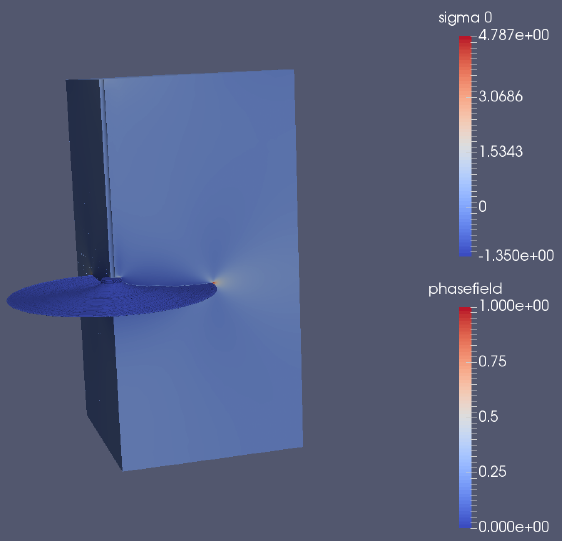
\includegraphics[width=0.3\textwidth]{figures/geomint-me3-01a.png}
\caption{Simulation von Bruchvorgängen mit der Phasenfeld-Methode \cite{Yoshioka2020}}
\label{fig:wp2}
\end{wrapfigure}
%\end{comment}
Die druckgetriebene Perkolation von Fluiden in einer geologischen Verwerfung im Tonstein wurde auf In-situ-Skala an Hand des Fault-Slip (FS) Experimentes im Felslabor Mt. Terri analysiert und mit Modellergebnissen, die durch der Lower-dimensional Interface Element (LIE) Methode gewonnen wurden, verglichen \cite{Vowinckel2020}. 
%
Darüber hinaus wurden Methoden zur Beschreibung der Ausbreitung von Fluiden auf den Grenzflächen polykristallinen Gesteins verfeinert und erweitert. Dies geschah in enger Wechselwirkung mit Laborversuchen, in denen Permeabilitäten, Rissschlie{\ss}ung und Verheilung unter unterschiedlichen Bedingungen mit Gas und Sole an Steinsalz und Tonstein gemessen wurden. Im Ergebnis konnten quantitative Voraussagen getroffen und das Spektrum an beschreibbaren Prozessen erweitert werden.

Ein systematischer Vergleich von verschiedenen Berechnungsmethoden (LIE, Phasenfeld-Methode, Non-Local Deformation) für druckgetriebene Perkolation wurde in \cite{Yoshioka2019} beschrieben.
%
Da sich Kriech- und Schädigungsprozesse im Steinsalz auf sehr unterschiedlichen Zeitskalen entwickeln und die Prozessbeschreibung auf stark nichtlinearen Gleichungssystemen beruht, wurde ein adaptives Zeitschrittverfahren für implizite FEM-Simulationen implementiert und anhand monotoner sowie zyklischer Belastungsversuche an Steinsalz getestet \cite{Zhang2020}. Mit dem Verfahren steigen sowohl die Effizienz als auch die Genauigkeit der Simulationen, wobei letztere durch den Nutzer sehr konkret mittels einer definierten oberen Fehlerschranke kontrolliert werden kann.
%
Alle o.g. numerischen Methoden wurden in die wissenschaftliche Open-Source-Software OpenGeoSys implementiert und stehen damit über die GeomInt-Modellierungsplattform zur Verfügung.

%======================================================================================
\section*{AP3: Wegsamkeiten durch Spannungsumlagerungen}
\label{sec:wp3}

Im Freiberger Geotechnik-Labor wurden die experimentellen Grundlagen zum Verständnis der Grundlagen für die Migration von Fluiden entlang von Diskontinuitäten in kristallinem Gestein mit unterschiedlichem Gefüge gelegt.
Um das Systemverständnis weiter zu verbessern, wurden Gesteine mit Variation der Korngrö{\ss}e (Kristallgrö{\ss}e) über mehrere Grö{\ss}enordnungen untersucht -- sehr grob-kristalliner Granit mit porphyrischem Gefüge bis zu fein-körnigem, dichtem Basalt. Die geometrischen Charakteristika sämtlicher Kluftflächen vor deren Belastung wurden mit einem 3D-Scanner flächenhaft erfasst und ausgewertet. 

%\begin{comment}
\begin{wrapfigure}{l}{0.45\textwidth}
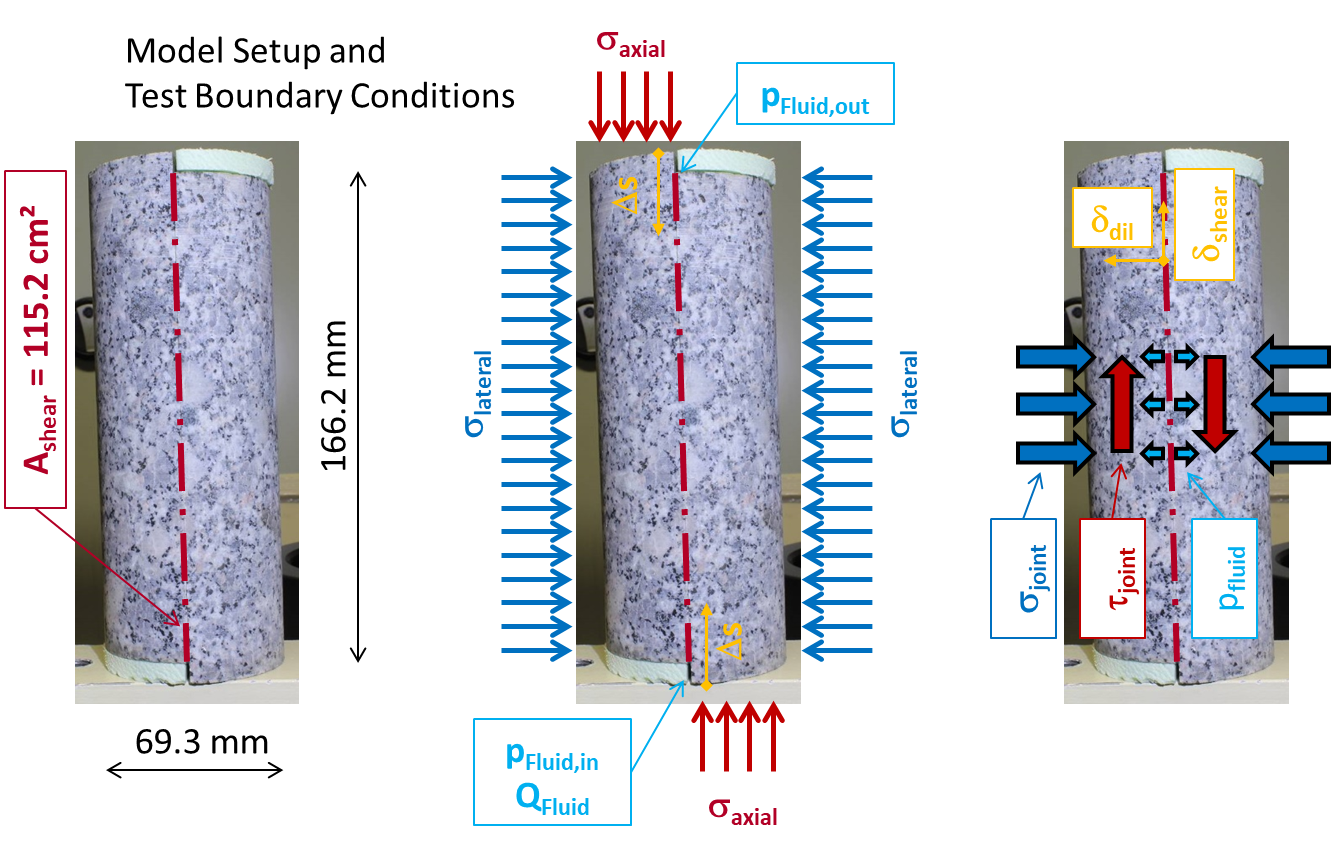
\includegraphics[width=0.45\textwidth]{figures/geomint-wp3-11.png}
\caption{Vorbereitung des Kernmaterials}
\label{fig:wp3-results-tubaf}
\end{wrapfigure}
%\end{comment}
Den Extremfall stellte jeweils eine makroskopisch glatte Kluft dar, die durch einen Sägeschnitt mit der Diamantkreissäge hergestellt wurde. 
Neben mechanischen Versuchsrandbedingungen mit konstanter Auflastspannung bei quasi-statischer Belastung und dynamisch-zyklischer Anregung wurden definierte Steifigkeiten des umgebenden Gebirges im Labor vorgegeben. Durch die Realisierung hydro-mechanisch gekoppelter Szenarien konnte die hydraulische Wirksamkeit der Diskontinuitäten unter den sich ändernden Spannungsrandbedingungen experimentell beobachtet werden. Der lokale Schädigungszustand der Probe wurde durch Scannen der Kluftflächen nach jedem Belastungsschritt dokumentiert. Im Ergebnis dieses klar definierten, mehrstufigen Vorgehens war es möglich, die experimentellen Grundlagen zur Abbildung typischer Belastungssituationen von potentiellen Wegsamkeiten im Kristallingestein zu schaffen.
Durch den Fokus auf gekoppelte mechanische und hydraulische Phänomene, die zum Teil aus dem Probematerial selbst (z.B. Korngrö{\ss}e, Kluftgeometrie, lokal unterschiedliche Festigkeiten, lokale Schädigung) zum Teil auch aus den Belastungsrandbedingungen (z.B. quasi-statisch vs. dynamisch, Steifigkeit des umgebenden Gebirges) herrühren, konnte das integrale Verhalten von Diskontinuitäten im kristallinen Gestein dokumentiert werden. 
%
Ein weiterer Schwerpunkt lag in der Entwicklung eines numerischen Algorithmus zur Berechnung von scherbeanspruchten Klüften im kristallinen Gestein. Da als wesentliche Modelleingangsparameter neben den makroskopischen Gesteinseigenschaften primär die geometrischen Eigenschaften der Kluftufer gewählt wurden, können sowohl konkrete Einzelsituationen nachgerechnet als auch das Verhalten von Diskontinuitäten prädiktiv abgeschätzt werden \cite{Poetschke2020}.
Der erstgenannte Fall dient zur Kalibrierung des numerischen Modells mit Hilfe der durchgeführten Laborversuche und zur Berechnung ausgewählter, gut dokumentierter Einzelfälle. Im zweitgenannten Fall können Sets von Klüften mit typischen Eigenschaften auf Basis geologischer Beobachtungen anhand statistisch generierter Parametersätze erstellt werden. 
Durch den sehr geringen Zeitaufwand zur Lösung einer Einzelberechnung ist das Modell gut geeignet das erwartbare Verhalten der Diskontinuitäten im Kristallin als Ergebnis einer Vielzahl von Einzelberechnungen zu ermitteln und (als Einhüllende) darzustellen. 
Mit diesem Ansatz können trotz unvermeidbarer statistischer Unsicherheiten hinsichtlich der konkreten Ausbildung der geometrischen und mechanischen Eigenschaften von geologischen Strukturen Aussagen zum Verhalten von Diskontinuitäten getroffen und in geotechnischen Studien berücksichtigt werden.

%\begin{comment}
\begin{wrapfigure}{l}{0.4\textwidth}
\vspace{-5mm}
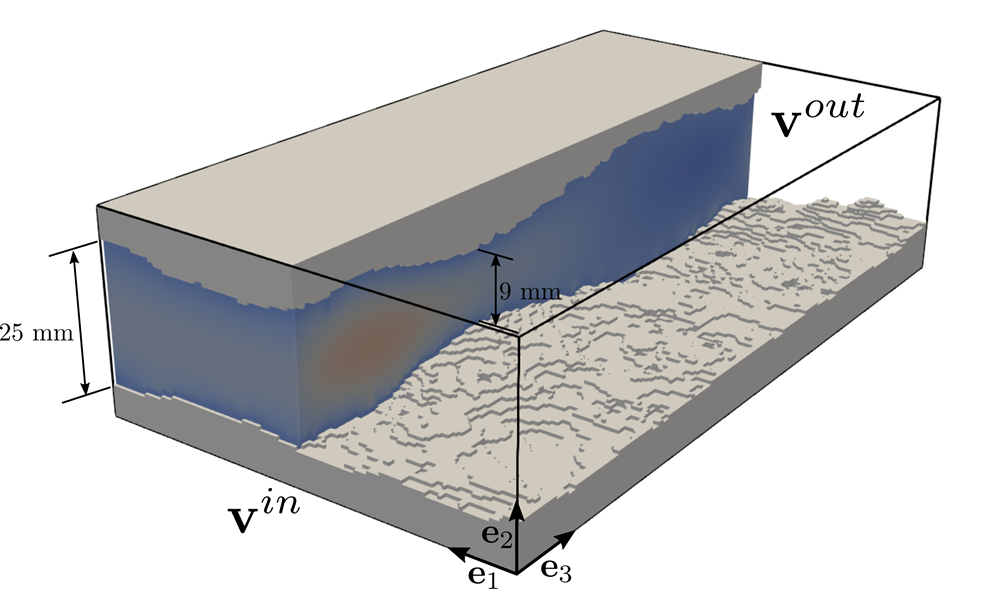
\includegraphics[width=0.4\textwidth]{figures/geomint-me08-01.png}
\caption{Strömungssimulation in Klüften mit der FEM \cite{steeb-2020c}}
\label{fig:wp3-results}
\end{wrapfigure}
%\end{comment}
%
Bezüglich der Modellierung wurde die hydro-mechanische Interaktion im kristallinen Gebirge (Granit, Gneis) mittels gekoppelten mehrskaligen numerischen Methoden (Smoothed Particle Hydrodynamics - SPH und Finite Elemente - FEM) analysiert. In kleinskaligen Untersuchungen einzelner Risse wurde gezeigt, dass der Effekt von Rissrauigkeiten Auswirkungen auf Transport- und Druckdiffusionsprozesse hat \cite{steeb-2019b}. Sind Rissgeometrie und Oberflächenrauigkeit bekannt, kann numerisch die effektive hydraulische Leitfähigkeit mit effizienten direkten numerischen Verfahren (SPH) mit hoher Genauigkeit berechnet werden \cite{steeb-2019b}. Im Rahmen der hybrid-dimensionalen FEM wurden die Rissrauigkeiten mittels eines neuen effektiven Spannungskonzept-Ansatzes integriert \cite{schmidt2019}.
Die numerische Effizienz und Genauigkeit wird dabei durch eine starke oder eine schwache Kopplung mittels nicht-konformen Netzen realisiert.
%
In hochauflösenden zeit-harmonischen Laborexperimenten konnte eine gute Übereinstimmung des Modells für nichtlineare Prozesse gezeigt werden, bei denen die hydraulische Leitfähigkeit stark von der Deformation des Risses einschlie{\ss}lich der Deformation von Kontaktflächen teilweise geschlossener Risse abhängt \cite{steeb-2020a}.
%
Schädigungs- und Bruchprozesse im Granit wurden mit nichtlokalen Ansätzen modelliert und konnten sowohl lokal aufgelöste als auch integrale Messgrö{\ss}en aus Dreipunktbiegeversuchen erfolgreich nachbilden, ohne dass ein gesondertes Anpassen der Materialparameter an diese Versuche nötig gewesen wäre \cite{Parisio2019102}.

Erste Übertragungen der Modelle auf die Feldskala, und damit die numerische Interpretation von transienten Pumpversuchen zur Charakterisierung der hydro-mechanischen Eigenschaften geklüfteter kristalliner Gesteinsformationen wurden in enger Kooperation mit den experimentellen Daten aus Pumpversuchen 
in Untertagelabors durchgeführt \cite{steeb-2020b} (In-situ-Stimulation and Circulation experiment - ISC, Grimsel Test Site) und \cite{steeb-2020c} (STIMTEC, Reiche Zeche, Freiberg).

\section*{Synthese}
\label{sec:syn}

Auf die Synthese von Experiment und Modell wurde von Anfang an gro{\ss}er Wert gelegt, daher wurden zu Beginn des Vorhabens sogenannte Modell-EXperimente (MEX) definiert.
Dabei handelt es sich um eine systematische, umfassende Untersuchung der zu Diskontinuitäten führenden Prozesse (Quellen/Schrumfen, Perkolation/Heilung, Spannungsumlagerung) durch die Kombination von Experiment und Modell.

\subsection*{Experimentelle Plattform}
\label{sec:exp}

Die experimentellen Analysen wurden bei den beteiligten Projektpartnern an unterschiedlichen Materialien durchgeführt. Die Untersuchungen am Tonstein, Steinsalz und dem kristallinen Gestein erforderten spezialisierte Laborexperimente. Standard-Triaxialversuche, um die Parameter im Versagenszustand zu bestimmen, können in allen Laboren in Freiberg, Leipzig und Kiel zu Vergleichszwecken durchgeführt werden.
Weitergehende Untersuchungen wurden in enger Absprache in den spezialisierten Labors durchgeführt.
%
Perkolationsversuche an zylindrischen Salzproben unter hydrostatischen und deviatorischen Bedingungen können im Leipziger sowie an Tonstein unter triaxialen Bedingungen in der Würfeldruckpresse im Kieler Labor durchgeführt werden. Dort erfolgten ebenfalls die Analyse des Quell- und Schrumpfverhaltens des Tonsteins unter verschiedenen Matrixspannungen sowie die Bestimmung der Bruchzähigkeit mittels Dreipunktbiegeversuch sowie der Zugfestigkeit aus Splitversuchen bei unterschiedlichen thermischen und hydraulischen Randbedingungen.
%
Die Analyse des Scherverhaltens von kristallinen Gesteinen in Fels-Rahmenscherversuchen erfolgte im Freiberger Labor. Für die kleinskalige Charakterisierung von Rissen in Gesteinsproben (typische Grö{\ss}en: $D=30$\,mm) wurde ein hochauflösendes Röntgentomographiegerät (XRCT) im Stuttgarter Labor verwendet. 
Die Oberflächen- und XRCT-Scans können für weiterführende  Untersuchungen in der Fortsetzung des Vorhabens weiter verwendet werden.
%
Die Zusammenarbeit der Projektpartner im experimentellen Bereich ist in der Abb. \ref{fig:appraoch} grafisch dargestellt - insbesondere die gegenseitige Bereitstellung und Aufbereitung des Probenmaterials aus den verschiedenen URLs für die geotechnischen Labore war ein erheblicher Mehrgewinn für die experimentelle Plattform in GeomInt.

\subsection*{Modellierungs-Plattform}
\label{sec:mod}
\begin{comment}
\begin{wrapfigure}{l}{0.42\textwidth}
\vspace{-5mm}
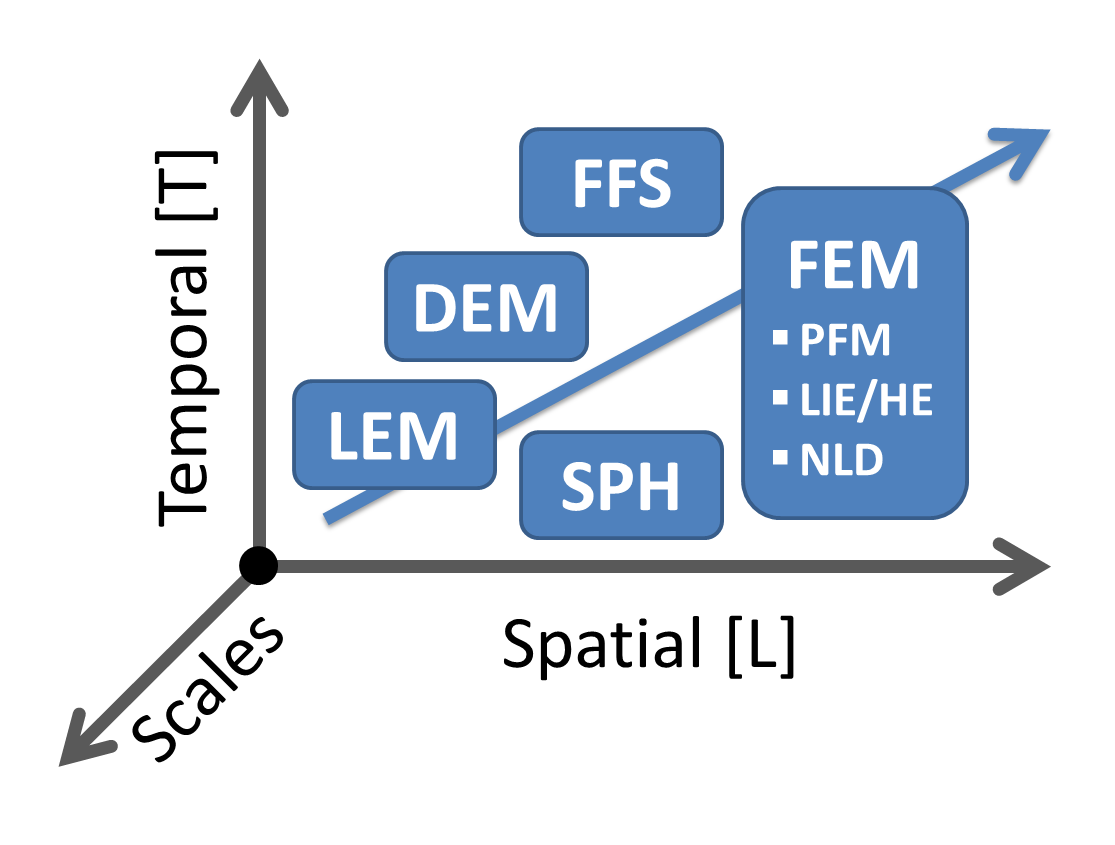
\includegraphics[width=0.4\textwidth]{figures/geomint-mod-scales1.png}
\caption{GeomInt-Modellierungsplattform}
\label{fig:mod-hub}
\end{wrapfigure}
\end{comment}
Ein wesentliches Ergebnis des GeomInt-Vorhabens ist die Entwicklung einer Modellierungsplattform. Dabei wurden verschiedene Modellierungskonzepte weiterentwickelt und verifiziert, die insbesondere die Evolution von Diskontinuitäten auf verschiedenen Raum-Zeit-Skalen abbilden können. In einer Reihe von Modell-EXperiment-Studien (MEX) wurden diese Konzepte für die verschiedenen Prozesstypen (AP1-AP3) miteinander verglichen (proof-of-concept), um die Vor- und Nachteile der einzelnen Methoden herauszuarbeiten \cite{Yoshioka2019}.
Ein besonderer Schwerpunkt lag in der Entwicklung von Open-Source-Software \cite{Bilke2019337}, um eine kontinuierliche Entwicklung der Plattform auch in der Zukunft zu gewährleisten. Zur Software-Entwicklung und \glqq best-practices\grqq{} wurde ein Workshop für alle \textsc{Geo:N} Verbundprojekte im April 2020 in Leipzig durchgeführt.
